% kmc_second_order.png: one step of second-order KMC (KineticMcChainOmpi), the sites and the paths it sums over.
% Make it in this folder with, for any scratch folder T:
%   pdflatex -output-directory=T fig_kmc_second_order.tex
%   python3 pdf_to_png.py T/fig_kmc_second_order.pdf ../kmc_second_order.png
\documentclass[11pt,tikz,border=1.5pt]{standalone}
% Shared preamble of all figures. Every fig_*.tex is compiled on its own, see the comment at its top; the fonts are those of the matplotlib
% style xzc_sans (amsmath, amssymb, amsfonts, sfmath), so that line drawings and data plots look the same.
\usepackage{amsmath,amssymb,amsfonts}
\usepackage{sfmath}
\renewcommand{\familydefault}{\sfdefault}
\usepackage{graphicx}
\usetikzlibrary{arrows.meta,calc,positioning,decorations.pathreplacing,backgrounds,shapes.geometric}
% species: Al gray, Mg orange, Zn blue; red marks the vacancy and the jumping atom
\definecolor{cAl}{HTML}{B8BCC2}
\definecolor{cMg}{HTML}{E08A2E}
\definecolor{cZn}{HTML}{3F78B5}
\definecolor{cOne}{HTML}{C8423B}
\definecolor{cTwo}{HTML}{3F78B5}
\definecolor{cThree}{HTML}{3E9B5C}
\definecolor{cFour}{HTML}{E0A21B}
\definecolor{cGray}{HTML}{7E858F}
\definecolor{cDark}{HTML}{2B2B2B}
\newcommand{\panel}[1]{\textbf{(#1)}}
\newcommand{\DM}{D_{\mathrm{MEP}}}
\newcommand{\KI}{K_{\mathrm{I}}}
\newcommand{\KF}{K_{\mathrm{F}}}
\newcommand{\dE}{\Delta E}
\newcommand{\Ea}{\Delta E_{\mathrm{a}}}
\newcommand{\ea}{\Delta e_{\mathrm{a}}}
\newcommand{\Ebind}{E_{\mathrm{bind}}^{\mathrm{site}}}
% a ball with a soft highlight, like the rendered spheres
\makeatletter
\pgfdeclareradialshading[tikz@ball]{softball}{\pgfpoint{-9bp}{9bp}}{%
  color(0bp)=(tikz@ball!22!white); color(6bp)=(tikz@ball!62!white); color(13bp)=(tikz@ball!96!white);
  color(20bp)=(tikz@ball!92!black); color(27bp)=(tikz@ball!74!black); color(50bp)=(tikz@ball!55!black)}
\makeatother
\tikzset{
  every picture/.append style={line cap=round, line join=round},
  every node/.append style={font=\small},
  img/.style={inner sep=0pt, anchor=south west},
  lab/.style={font=\normalsize, inner sep=1pt, anchor=north west},
  above lab/.style={font=\normalsize, inner sep=1pt, anchor=south west},
  capt/.style={align=center, anchor=north},
  atom/.style={circle, ball color=#1, shading=softball, minimum size=12pt, inner sep=0pt},
  atom/.default=cAl,
  vac/.style={circle, draw=cOne, line width=1.1pt, fill=white, minimum size=11.5pt, inner sep=0pt},
  arr/.style={-{Stealth[length=5pt]}, line width=0.8pt},
  dbl/.style={{Stealth[length=4pt]}-{Stealth[length=4pt]}, line width=0.8pt},
  jump/.style={arr, cOne, line width=1.2pt},
  block/.style={-{Triangle[length=8pt, width=13pt]}, line width=5pt, cTwo!38},
  cell axis/.style={-{Triangle[length=6pt, width=5.5pt]}, line width=1.2pt, black},
  dir/.style={fill=white, fill opacity=0.75, text opacity=1, font=\footnotesize, inner sep=1.5pt},
}
\graphicspath{{img/}}
% data plots are included at one scale: \plot{name}{x}{y}{file}
\newcommand{\plotscale}{0.6}
\newcommand{\plot}[4]{\node[img] (#1) at (#2,#3) {\includegraphics[scale=\plotscale]{#4}};}
\newcommand{\plotlabel}[2]{\node[above lab] at ($(#1.north west)+(-0.05,0.02)$) {\panel{#2}};}
% legend of the species, first entry at (#1,#2): Al, Mg, Zn (and the vacancy)
\tikzset{leg/.style={anchor=base west, inner sep=2pt, yshift=-3.2pt}}
\newcommand{\specieslegend}[2]{%
  \foreach \lx/\lc/\lt in {0/cAl/Al, 1.2/cMg/Mg, 2.4/cZn/Zn} {
    \node[atom=\lc, minimum size=10pt] at ({#1+\lx},#2) {}; \node[leg] at ({#1+\lx+0.2},#2) {\lt};}}
\newcommand{\vacancylegend}[2]{\node[vac, minimum size=9.5pt] at (#1,#2) {}; \node[leg] at ({#1+0.2},#2) {vacancy};}

\begin{document}
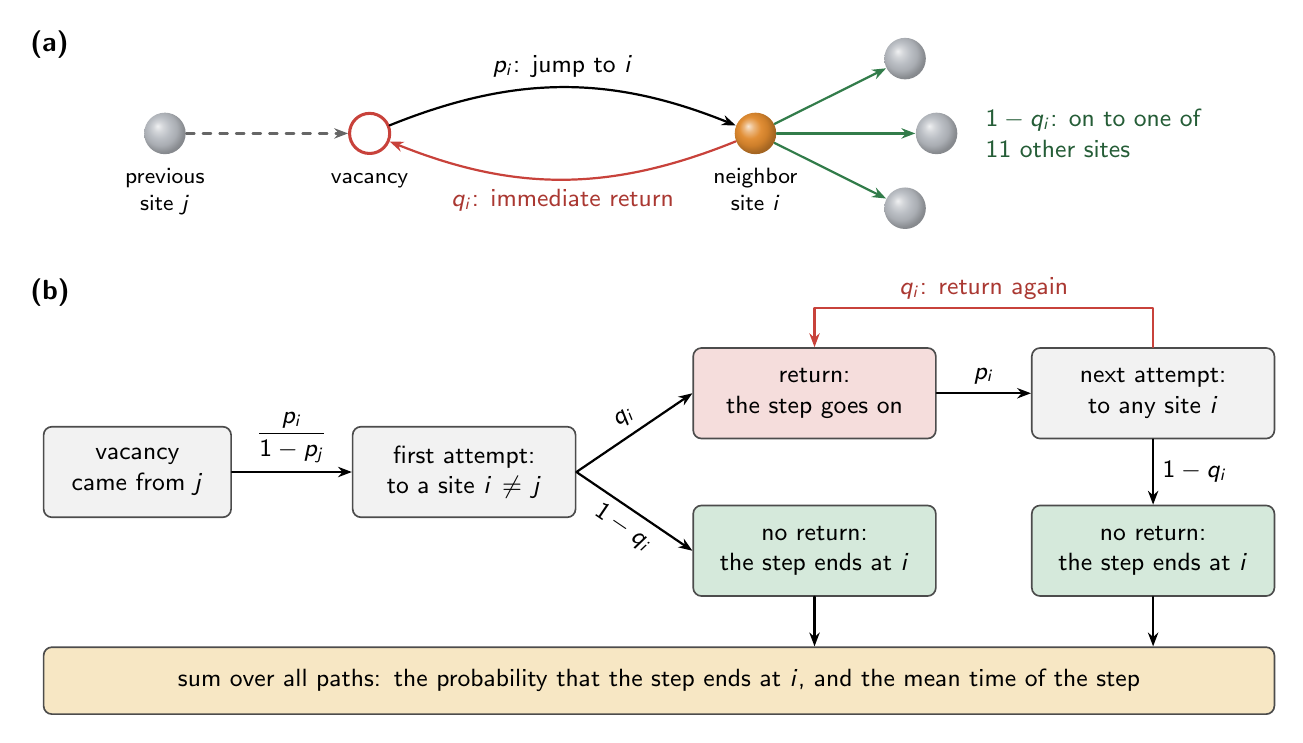
\begin{tikzpicture}[
    st/.style={atom=#1, minimum size=15pt}, st/.default=cAl,
    box/.style={draw=black!70, rounded corners=3pt, align=center, inner sep=4pt, fill=black!5, minimum height=1.15cm, line width=0.6pt},
    endbox/.style={box, fill=cThree!22},
    backbox/.style={box, fill=cOne!18},
    sumbox/.style={box, fill=cFour!26, minimum height=0.85cm},
    site/.style={font=\footnotesize, align=center, anchor=north, inner sep=0pt},
    pr/.style={font=\small, inner sep=3pt}]
  % ---------------- (a) sites and probabilities ----------------
  \begin{scope}[shift={(0.45,0)}]
    \node[st] (j) at (0,0) {};
    \node[vac, minimum size=14.5pt] (k) at (2.6,0) {};
    \node[st=cMg] (i) at (7.5,0) {};
    \node[st] (l1) at (9.4,0.95) {};
    \node[st] (l2) at (9.8,0) {};
    \node[st] (l3) at (9.4,-0.95) {};
    \draw[arr, dashed, black!60] (j) -- (k);
    \draw[arr] (k) to[bend left=22] node[above] {$p_i$: jump to $i$} (i);
    \draw[arr, cOne] (i) to[bend left=22] node[below, text=cOne!85!black] {$q_i$: immediate return} (k);
    \draw[arr, cThree!80!black] (i) -- (l1);
    \draw[arr, cThree!80!black] (i) -- (l2);
    \draw[arr, cThree!80!black] (i) -- (l3);
    \node[text=cThree!60!black, anchor=west, align=left] at (10.3,0) {$1-q_i$: on to one of\\ 11 other sites};
    \node[site] at (0,-0.40) {\strut previous\\ \strut site $j$};
    \node[site] at (2.6,-0.40) {\strut vacancy};
    \node[site] at (7.5,-0.40) {\strut neighbor\\ \strut site $i$};
    \node[lab] at (-1.75,1.35) {\panel{a}};
  \end{scope}
  % ---------------- (b) paths ----------------
  \begin{scope}[shift={(0,-4.3)}]
    \node[box, text width=2.1cm] (A) at (0.1,0) {vacancy\\ came from $j$};
    \node[box, text width=2.55cm] (B) at (4.25,0) {first attempt:\\ to a site $i\neq j$};
    \node[backbox, text width=2.8cm] (D) at (8.7,1.0) {return:\\ the step goes on};
    \node[endbox, text width=2.8cm] (C) at (8.7,-1.0) {no return:\\ the step ends at $i$};
    \node[box, text width=2.8cm] (E) at (13.0,1.0) {next attempt:\\ to any site $i$};
    \node[endbox, text width=2.8cm] (F) at (13.0,-1.0) {no return:\\ the step ends at $i$};
    \draw[arr] (A) -- node[pr, above] {$\dfrac{p_i}{1-p_j}$} (B);
    \draw[arr] (B.east) -- node[pr, above, sloped] {$q_i$} (D.west);
    \draw[arr] (B.east) -- node[pr, below, sloped] {$1-q_i$} (C.west);
    \draw[arr] (D) -- node[pr, above] {$p_i$} (E);
    \draw[arr] (E) -- node[pr, right] {$1-q_i$} (F);
    \draw[arr, cOne] (E.north) -- ++(0,0.5) -| node[pos=0.25, above, text=cOne!85!black, inner sep=2.5pt]
         {$q_i$: return again} (D.north);
    \node[sumbox, text width=15.35cm] (S) at (6.725,-2.65)
         {sum over all paths: the probability that the step ends at $i$, and the mean time of the step};
    \draw[arr] (C) -- (C.south |- S.north);
    \draw[arr] (F) -- (F.south |- S.north);
    \node[lab] at (-1.3,2.5) {\panel{b}};
  \end{scope}
\end{tikzpicture}
\end{document}
